%%%%%%%%%%%%%%%%%%%%%%% file typeinst.tex %%%%%%%%%%%%%%%%%%%%%%%%%
%
% This is the LaTeX source for the instructions to authors using
% the LaTeX document class 'llncs.cls' for contributions to
% the Lecture Notes in Computer Sciences series.
% http://www.springer.com/lncs       Springer Heidelberg 2006/05/04
%
% It may be used as a template for your own input - copy it
% to a new file with a new name and use it as the basis
% for your article.
%
% NB: the document class 'llncs' has its own and detailed documentation, see
% ftp://ftp.springer.de/data/pubftp/pub/tex/latex/llncs/latex2e/llncsdoc.pdf
%
%%%%%%%%%%%%%%%%%%%%%%%%%%%%%%%%%%%%%%%%%%%%%%%%%%%%%%%%%%%%%%%%%%%
\documentclass[runningheads,a4paper]{llncs}

\usepackage{amssymb}
\setcounter{tocdepth}{3}
\usepackage{graphicx}
\usepackage{color}
\usepackage{tabularx}
\usepackage{nameref}
\usepackage[hidelinks]{hyperref}
\usepackage{subfigure}
%\usepackage[titletoc]{appendix}

% For nice code highlighting
\usepackage{listings}
\usepackage{xcolor}
\colorlet{punct}{red!60!black}
\definecolor{background}{HTML}{EEEEEE}
\definecolor{delim}{RGB}{20,105,176}
\colorlet{numb}{magenta!60!black}
\colorlet{comment}{green!60!black}
\lstdefinelanguage{survey}{
    basicstyle=\normalfont\ttfamily,
    numbers=left,
    numberstyle=\scriptsize,
    stepnumber=1,
    firstnumber=0,
    numbersep=8pt,
    showstringspaces=false,
    breaklines=true,
    frame=single,
    language=C++,
    xleftmargin=2em,
    framexleftmargin=1.5em,
    backgroundcolor=\color{background},
    stringstyle=\color{delim},
    literate=
     *{Survey}{{{\color{numb}Survey}}}{5}
     {Intro}{{{\color{numb}Intro}}}{4}
     {Question}{{{\color{numb}Question}}}{7}
     {TableQuestion}{{{\color{numb}TableQuestion}}}{11}
     {exclusive}{{{\color{numb}exclusive}}}{7}
     {optional}{{{\color{numb}optional}}}{7}
     {Answer}{{{\color{numb}Answer}}}{4}
     {->}{{{\color{numb}->}}}{2}
     {Items}{{{\color{numb}Items}}}{3}
     {freetext}{{{\color{numb}freetext}}}{7}
     {Outro}{{{\color{numb}Outro}}}{4},
     morecomment=[s][\color{comment}]{/*}{*/}
}

\usepackage{url}
\urldef{\mailsa}\path|{tebr, nmar, tmis, cosm}@itu.dk|
\newcommand{\keywords}[1]{\par\addvspace\baselineskip
\noindent\keywordname\enspace\ignorespaces#1}

\begin{document}

\mainmatter  % start of an individual contribution

% first the title is needed
\title{Domain-specific Language for Hierarchical Survey Construction}

% a short form should be given in case it is too long for the running head
\titlerunning{Domain-specific Language for Hierarchical Survey Construction}

% the name(s) of the author(s) follow(s) next
%
% NB: Chinese authors should write their first names(s) in front of
% their surnames. This ensures that the names appear correctly in
% the running heads and the author index.
%
\author{Theresa Brandt von Fackh\and Niels Martin S{\o}holm\and Tomas Miseikis\and Cosmin Catalin Sanda}
%
\authorrunning{Domain-specific Language for Hierarchical Survey Construction}
% (feature abused for this document to repeat the title also on left hand pages)

% the affiliations are given next; don't give your e-mail address
% unless you accept that it will be published
\institute{Model Driven Development Project\\IT University of Copenhagen\\
\mailsa}

%
% NB: a more complex sample for affiliations and the mapping to the
% corresponding authors can be found in the file "llncs.dem"
% (search for the string "\mainmatter" where a contribution starts).
% "llncs.dem" accompanies the document class "llncs.cls".
%

\toctitle{Domain-specific Language for Hierarchical Survey Construction}
\tocauthor{Theresa Brandt von Fackh, Niels Martin S{\o}holm, Tomas Miseikis and Cosmin Catalin Sand}
\maketitle

\begin{abstract}
In this project a domain-specific language for hierarchical survey construction has been implemented. The language is targeted towards survey developers in psychology and general medical-oriented statistics. Moreover, three code generators have been implemented that can generate web applications, Android apps and DOT graph survey diagrams respectively.
\end{abstract}

\section{Background}
\label{sec:background}
A survey is a set of questions presented to people (respondents) in order to collect facts and/or opinions. It is a technique employed throughout various academic disciplines (e.g. psychology) as well as a number of commercial domains (e.g. marketing) that collect data~\cite{synodinos}. Though the technique, in its physical form, has been practiced for hundreds of years, it is only in recent decades that disciplines such as cognitive psychology and linguistic pragmatics have been applied to make the field of survey construction into a science rather than an art~\cite{martin}.

Research has shown that answers to questions of a survey may be subject to ``context effects" caused by subsequent questions. In other words, question sequence can have an impact on the outcome of a survey~\cite{synodinos,johnson,martin}. Various motivators or ``types" of context effects have been hypothesized. For example ``attitude crystallization", which refers to a case where the respondents' opinion regarding a specific topic develops, as they have discussed or thought more thoroughly about the topic. The respondents form a definite, ``crystallized" opinion~\cite{johnson}. Aside from attitude crystallization, a number of other motivators have been hypothesized. It is beyond the scope of this report to delve deeper into these, but suffice to say that question sequence is a relevant concern. 

Modern surveys tend to be delivered online and are self-administered by the respondent. They lack the sense of length and overview a traditional pen and paper survey provides. Due to this, and possible other factors, the risk of partial completion is much more likely~\cite{lumsden_morgan}. Research suggests that proper question sequencing may affect the rate of partial completion. For example, asking personal or complex questions in the very beginning of a survey may cause the respondent to quit~\cite{lumsden_morgan}.

One of the techniques to improve response quality as well as reduce risk of partial completion is branching/hierarchical surveys. They let the question sequence be determined in real-time based on the answers of the respondent. Often groups of respondents will be hypothesized and the branching of questions will seek to lead certain groups towards certain questions. This can be exploited to ask the right questions in the right way. Adaptive surveys like these have been used by psychologists as well as for general medical statistics~\cite{schouten}.

\section{Project Description}
\label{project_description}
In order to accommodate the above we suggest an external domain-specific language (DSL) for survey construction. The target users of the language (survey developers) are psychologists or general medical statisticians. The target users of the generated survey applications (respondents) could be anyone. We choose external DSL, because we expect the survey developers to have limited programming experience. To support this we need a simple language and environment that only makes use of few basic and domain-related concepts. Furthermore, the environment should ease hierarchical survey construction by providing an overview of the numerous execution paths, allowing the survey developer to assert the risk of context effects and the general flow of the survey.

We have defined the following requirements:
\begin{itemize}
	\item Tooling requirements:
	\begin{itemize}
		\item An interactive development environment (IDE) with syntax highlighting and a static checker.
		\item A generator capable of generating computerized surveys (Android app \& web page) to be interacted with directly by respondents.
		\item A generator capable of generating question sequencing (flow diagram) to be used by survey developers during survey construction.
	\end{itemize}
	\item Language semantic requirements:
	\begin{itemize}
		\item Surveys should have an intro and an outro. Texts/pages shown to the respondent before and after survey completion.
		\item Optional questions should be possible, allowing the respondent to skip such questions.
		\item Free text answers should be possible, allowing the respondent to give a custom response.
		\item Both exclusive and non-exclusive questions should be possible, allowing the respondent to choose one or multiple answers depending on the given type of question.
		\item Questions with sub-items should be possible. Such as ``How do you like the following cities on a scale from 1 to 5?" and then the sub-items may be ``London", ``Copenhagen" and ``Paris". These can also be exclusive or non-exclusive, as well as optional.
		\item Support for branching surveys. It should be possible to construct questions that may lead the respondent to different follow-up questions depending on their choice of answer.
	\end{itemize}
\end{itemize}

\section{Architecture}
\begin{figure}[htb]
	\centering
	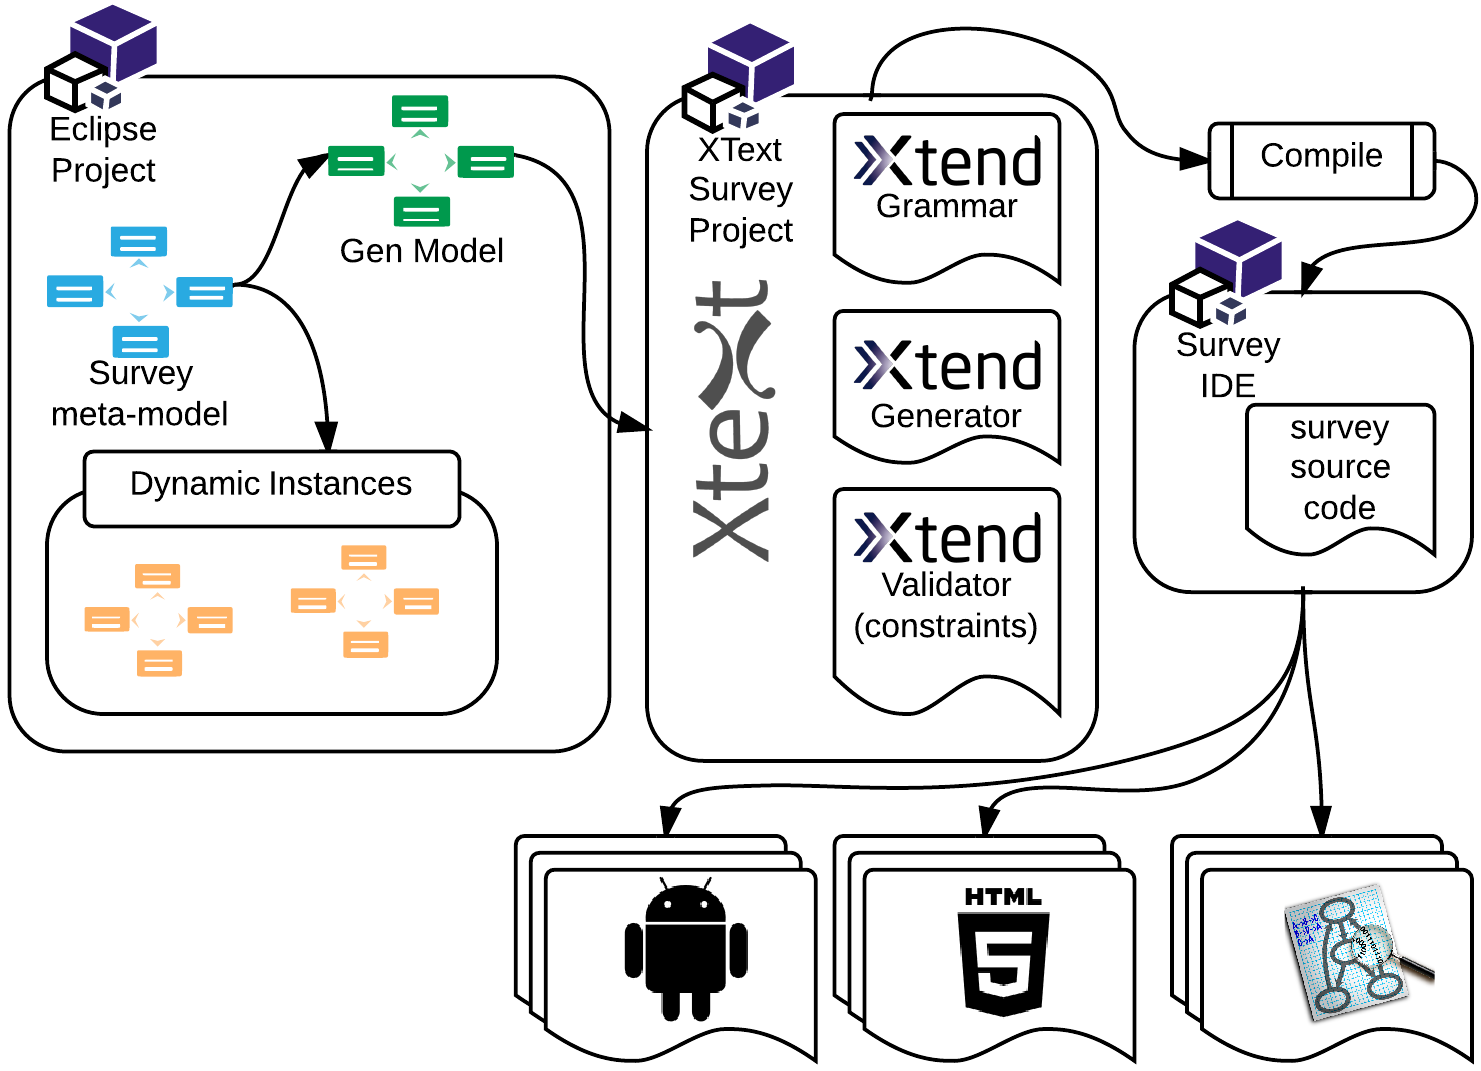
\includegraphics[scale=0.23]{images/survey_dsl_architecture}
	\caption{Survey system architecture}
	\label{fig:survey_system_architecture}
\end{figure}

\subsection{Eclipse Modeling Framework}
The architecture of the Survey generation system revolves around the Eclipse IDE\footnote{Eclipse is an integrated development environment (IDE). It contains a base workspace and an extensible plug-in system for customizing the environment (www.eclipse.org).}.
The first part of the system is composed of an Eclipse Modeling Framework (EMF) project in which the meta-model for the survey is defined. In the initial stages of development, the meta-model was tested with the help of dynamic instances. The sample instances help to detect logical issues early in the development process. Using the capabilities of EMF, we have generated the necessary files that are then used as input for the Xtext\footnote{Xtext is an open-source framework for development of programming langauges and domain-specific languages (www.eclipse.org/xtext).} framework.
Based on the EMF project we generated  the Xtext project in which the grammar, the validation and the code generators are defined. All of these three components are defined using Xtend\footnote{Xtend is a flexible and expressive dialect of Java, which compiles into readable Java 5 compatible source code (www.eclipse.org/xtend).}. The custom Xtend validations help the developer when writing the survey. The validations describe logical constraints for the model, which are enforced in the survey editor.

\subsection{Code Generators}
The surveys are generated for two platforms: web applications and Android. The surveys can have deep branching, which is better for display on digital mediums such as computers and mobile devices. Digital mediums, as opposed to physical paper, can automatically toggle questions based on the branching. Additionally, the Android based surveys coupled with web application surveys can potentially cover a significant proportion of respondents by using different digital channels.  On the downside, respondents who do not use Android devices or computers cannot be targeted by our tool. However, other generators can easily be added so that they can produce PDF or text based surveys.

We also use a third type of code generator which produces DOT graphs\footnote{DOT is a plain text graph description language. It is a simple way of describing graphs that both humans and computer programs can use (en.wikipedia.org/wiki/DOT{\_}(graph{\_}description{\_}language)).} of the surveys. The graphical representation of the DOT files can be used by the survey developer to better understand the structure and the branching of the generated surveys. Graphical representation are in general easier to understand for humans~\cite{karsai}. A representation of an example survey is shown in~\ref{fig:survey_graph} (Appendix).

The current three code generators are independent of each other. However, because the mediums for the survey have the same high level abstractions, no further processing needs to be made to accommodate different types of questions (this can be a problem when outputting surveys on paper for example, where conditional statements are hard to express). Another advantage of the currently chosen mediums is the possibility of sharing the back-end in which survey results are collected.
The Survey Xtext project is run as an Eclipse project, therefore creating the IDE in which the survey developer defines the surveys. The IDE has all the basic features like syntax highlighting and syntax errors. The errors are identified using the validation constraints. 

\section{Language Design}
In this chapter the meta-model, validation constraints and concrete syntax will be presented. Specific design decisions will be discussed. Arguments backed by design guidelines for domain-specific languages (DSL)~\cite{karsai} as well as the domain considerations will be made.

\subsection{Meta-Model}
\label{sec:meta_model}
The following meta-model provides the formal definition of the language we have created. It defines the abstract syntax for the language, which fulfills the requirements described in the project description (Chapter~\ref{project_description}). The meta-model is presented in Figure~\ref{fig:meta_model} as EMF Ecore Diagram.

\begin{figure}[htb]
	\centering
	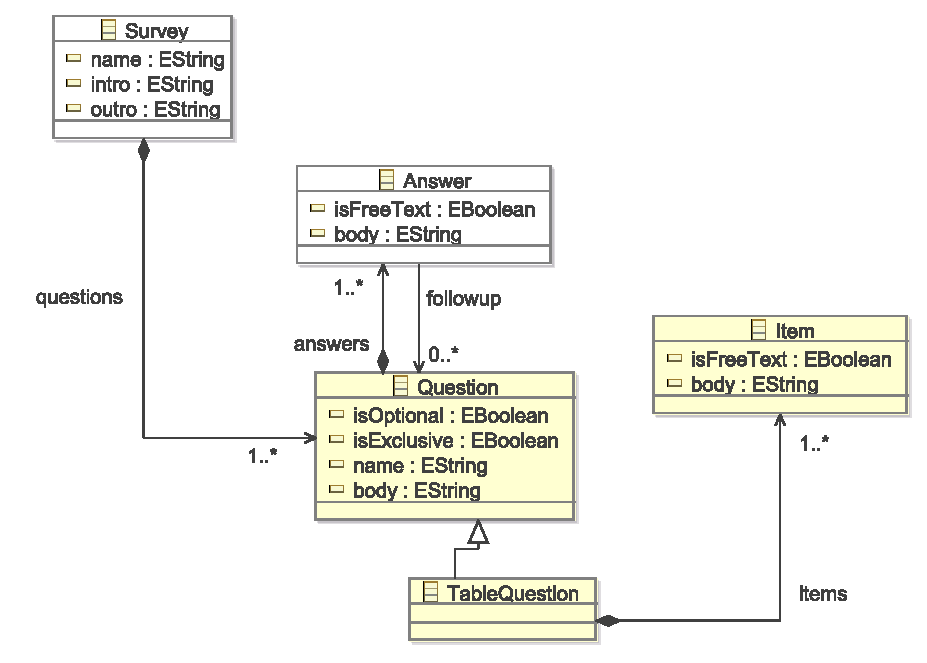
\includegraphics[scale=0.77]{images/meta_model}
	\caption{Ecore Diagram of the meta-model}
	\label{fig:meta_model}
\end{figure}

When modeling the meta-model for our language we started to define the main domain artifacts of a survey as classes and connecting these with respective relations. These main domain artifacts are:
\begin{itemize}
	\item \textit{\textbf{Survey}}, which encloses the whole structure of a survey
	\item \textit{\textbf{Question}}, which encloses a question and its answers in a survey
	\item \textit{\textbf{Answer}}, which contains one answer of a question
\end{itemize}

In the following paragraphs we describe the elaboration of this basic model to the actual meta-model for our language, which fulfills all the requirements of our project description, with respect to the design guidelines for DSLs~\cite{karsai}. 

We introduced another class \textbf{Content} to build a generalization of classes, which have a string text as attribute. These classes are \textbf{Question}, \textbf{Answer} and \textbf{Item}. The idea was to follow the guideline for avoiding redundancy~\cite{karsai}, by just using one field in one class instead of using the same field in several classes. But the advantage of reducing redundancy is not fully exploited by a simple string field. In comparison with the disadvantage of introducing more complexity in the model by this generalization and to keep the model simple~\cite{karsai}, we inserted the idea of the content by adding a field in each of the classes, where it is needed.

To configure the two segregative types of questions - exclusive and nonexclusive questions - we introduced a boolean attribute \textbf{isExclusive} on the class \textbf{Question}. Alternatively we could have made two subclasses of an overall class \textbf{Question} for these types. This way the model can be easily expanded, when introducing new types of questions, which are segregative from the existing types. But since class \textbf{TableQuestion} (discussed later on) is introduced as additional type of question and can be also of the type exclusive or nonexclusive, those types are inserted as boolean fields into the \textbf{Question} class, avoiding unnecessary generality~\cite{karsai}. Because otherwise the class \textbf{TableQuestion} has to be a subclass of each of these classes.

An answer can contain a follow-up question. Two concepts of introducing follow-up questions to an answer were discussed: reference or containment. The advantage of using a follow-up question as containment is that the survey developer does not have to reference a question by using some kind of ID. The concept of references might be familiar to people with IT-Background, but it can not be expected that non-IT people instantly know how to use references. It is also easier to read by the survey developer since the follow-up questions are included within the answer, while with references all follow-up questions will probably be at another place in the survey file. Such details can be challenging for the survey developer, who is not familiar with references as a concept. Furthermore infinite loops (Question A $\to$ Question B $\to$ Question C $\to$ Question B) can be avoided without introducing constraints. The disadvantages of using containment are that follow-up questions can not be reused, which might be cumbersome for the survey developer if the same question should be reused. We eventually sided with references due to the advantage of re-usability.

Another discussion was to introduce a boolean field to class \textbf{Question} to mark a it as follow-up question. For the survey developer it would be easier to explicitly indicate a question, which is used as follow-up question. A question could be used as follow-up question and as a regular question. But since we think it is unlikely that a survey developer would want to repeat a follow-up question as a regular question, we decided to not introduce another field. This would also complicate the model even more. A follow-up question can be identified as such by verifying if it is referenced by an answer.

\phantomsection
\label{par:table_questions}
To support questions with sub-items we introduce a subclass to the class Question called \textbf{TableQuestion}. The configurations of exclusive, non-exclusive, optional and non-optional could also apply for a \textbf{TableQuestion}, therefore an inheritance could be used to avoid redundancy~\cite{karsai}. Thus the question class can be expanded to different kind of questions without using redundant fields. Another possible solution would be to insert items directly to the question class and let the code generator handle the representation: If the question contains at least one item, it is handled as a \textbf{TableQuestion}. The disadvantage of this solution is redundant fields, that may increase if the fields for specific question types are added to the Question class instead of using own classes for the several question types, which are subclasses of the class Question. Table questions should not have follow-up question to reduce the complexity for the survey developer. This is secured by using constraints (Chapter~\ref{sec:constraints}). By introducing this constraint also the complexity for our grammar will be reduced since a follow-up question has to be applied to a single answer of a single item.

We first had a specific intro and the outro as containment of the survey class, but decided to include the intro and outro as attributes on the survey class instead. The intro and outro are strings, in which the survey developer can add a text. A dedicated class for intro and outro did not add a lot of value since no other functionality on an intro and outro is needed.

\section{Validation Constraints}
\label{sec:constraints}
Xtext incorporates syntactical validation, cross-link validation and concrete-syntax validation~\cite{xtext_doc}. In addition, we have implemented a number of our own custom validation constraints. The reason we have chosen to implement these constraints is because it is often argued that the best practice is to do as little as possible in the grammar and as much as possible in validation~\cite{bettini}. This allows to detect problems more precisely and provide better error messages. Whenever one or several rules are broken, the IDE generates an error, informing which rule or rules have been broken. This feedback can be crucial to the new users of our language, since it may lack a proper documentation. Furthermore, the default Xtext error messages given to the user may sound overly technical, making it hard to understand what went wrong.
Some of the validation rules that have been created for the Survey project are:

\begin{itemize}
	\item \textbf{Unique name validator.} It is reasonable to enforce the uniqueness of question names, since questions are referenced by their name.
	\item \textbf{Exclusive validator.} This ensures that all exclusive questions have at least two answers. 
	\item \textbf{TableQuestion has no followups validator.} As it was mentioned earlier, due to the complexity it would induce on the user, table questions are not allowed to have follow-up questions in their answers.
	\item \textbf{Cycle validator.} This prevents user to introduce cycles. Selecting a particular answer in one question can trigger a followup question to be shown after it. However, this followup question might have an answer that triggers the original question to be shown again, thus introducing a cycle. 
\end{itemize}

\section{Concrete Syntax}
The concrete syntax is used to define instances of the model. It is heavily influenced by the semantics of the model, however certain design decisions are entirely about concrete textual syntax. Despite the fact that the different syntactical solutions are not semantic in nature and the exact same abstract instances could be produced regardless of the chosen syntax, we argue that the choices are likely to have an impact in terms of how useful the language will be to the survey developers. In the following, a number of the most prominent syntactic decisions are discussed based on the example in Figure~\ref{fig:complete_survey_example}.

\begin{figure}[htb]
\begin{lstlisting}[language=survey]
Survey "A complete demo"

Intro "This survey demonstrates capabilities built into the survey Generator."

Question ORANGESIZE exclusive optional "How big do you like your oranges?"
(
	Answer "Large" /* Who really like oranges */
	Answer "Small"
)

Question FAVFRUITS "Which of the following fruits do you enjoy eating?"
(
	Answer "Apples"
	Answer "Oranges" -> ORANGESIZE
	Answer "Bananas"
	Answer freetext "Other fruits you like"
)

TableQuestion FOOTRATE exclusive "Rate the following football teams"
(
	Items ( "Looser", "Mediocre", "Winner" )
	Answer "Liverpool F.C."
	Answer "Juventus Torino"
	Answer "Getafe CF"
)

Outro "Thank you for taking the time to fill in our survey."
\end{lstlisting}
\caption{A complete survey example}
\label{fig:complete_survey_example}
\end{figure}

\subsection{Question attributes (exclusive and optional)}
Questions can optionally be declared exclusive and/or optional (see meta-model discussion for semantic clarification in Chapter~\ref{sec:meta_model}). They are a part of the initial textual description of a question (See lines 4 and 18 in Figure~\ref{fig:complete_survey_example}).

We discussed various representations. For example we considered the attribute ``optional" to be represented as: ``optional", ``opt" or ``?". We had to weigh compactness against comprehensibility. The longer full spelling of the attribute enhances readability, however the shorter versions would improve the productivity of the survey developer~\cite{karsai}. In such a case the frequency of the element should be a deciding factor~\cite{karsai}. We looked at some realistic survey samples and judged that the frequency compared to keywords such as \textbf{Question} and \textbf{Answer} is pretty low. Furthermore, it could be argued that the longer version is more descriptive. Descriptive notation increases learnability and comprehensibility of a language~\cite{karsai}. We considered the target survey developers (with limited programming experience) and agreed that those characteristics should be prioritized over developer's productivity.

\subsection{Parenthesis for list-like structures}
The language contains various list-like structures such as answers to a question or sub-items of a table question (See lines 4-8 and 20 in Figure~\ref{fig:complete_survey_example}). We have decided to wrap such lists in parenthesis, instead of brackets ``[", and curly-braces ``\{". The latter 2 symbols are very programming-centric and not necessarily common to the survey developers. We seek to adopt notations that we assume domain experts already feel the most familiar with. This way we enhance familiarity and reduce the learning barrier~\cite{karsai}.

\subsection{Answer and item redundancy in table questions}
In table questions we use answers and sub-items. Items are sub-parts of the question and are presented to the respondent together, usually as rows in a table. All the defined answers apply to all the defined items of the given question. The very basic syntactic approach would be to require answer options to be defined for every item as shown in~\ref{fig:tablequestion_redundancy} (Appendix).

This would increase redundancy at the cost of survey developer's efficiency.  Alternatively, a syntax in the form of single item and answer definitions could be considered (See lines 20-23 in Figure~\ref{fig:complete_survey_example}). Syntactic sugar like this does not contribute to the expressiveness of the language but improves readability~\cite{karsai}. On other hand, it diverges from the original ``style" of question definitions. Adopting a similar look-and-feel throughout a language increases understandability and can make it possible for the user to get a general intuition about the language~\cite{karsai}. Despite this argument we still feel the efficiency and readability gain of the addition is worth it.

\subsection{Question definition keywords}
Regular questions and questions with sub-items are defined with their respective keywords: \textbf{Question} and \textbf{TableQuestion}. This is not a parser requirement, a perfectly valid alternative would be to infer the question type based on its body (answers, items). We decided to stick to the keywords in order to enhance distinguishability. Easily distinguishable elements increase understandability~\cite{karsai}. The argument for absence of basic keywords is developer efficiency~\cite{karsai}. This is a weak argument in this context considering how tiny a fraction of a question definition the keyword represents.

\section{Testing}
We have validated our language by constructing 22 sample implementations in the concrete syntax itself. Each sample is tailored to test a specific language requirement or constraint. The samples are loaded by individual unit tests and compiled to an in-memory instance of the meta-model. In the positive tests the correctness of the model instance is validated with regards to the expected behavior in the particular test. In the negative tests, where the syntax is incorrect, a successful test run is one where the compiler fails.

A table containing an overview of all the unit tests can be found in Table~\ref{tbl:test_cases} (Appendix).

\section{Conclusion}
We have constructed a domain-specific language for hierarchical survey generation. It has tooling to aid survey construction, as well as generate dedicated survey applications to be used by respondents. It fulfills the stated semantic language requirements. The implementation of each requirement and constraint has been validated through unit tests.

\section{Future Work}
An improvement would be to provide a graphical concrete syntax instead of the textual representation. Since sequencing is an important aspect of creating surveys (Chapter~\ref{sec:background}) and graphical user interfaces are more convenient and understandable for the survey developer~\cite{karsai}, a graphical concrete syntax would make sense. We respected the importance of a graphical representation by providing a DOT Generator (Figure~\ref{fig:survey_graph} in Appendix). However it is not as efficient as allowing the user to edit the diagram directly. A complete graphical representation was out of scope of this project.

Many of the design arguments throughout the report are based on assumptions about the domain. We discussed a more thorough domain analysis with usability tests and/or interviews. We agreed that it was beyond the scope of the course, however in a real-world project this would be the right thing to do in order to verify our assumptions.

\begin{thebibliography}{4}

\bibitem{synodinos} Synodinos - 2002 - The Art of Questionnaire Construction
\bibitem{martin} Martin - 2006 - Survey Questionnaire Construction
\bibitem{johnson} Johnson et al. - 1998 - Effects of Question Context and Response Order on Attitude Questions
\bibitem{lumsden_morgan} Lumsden \& Morgan - 2005 - Online-Questionnaire Design: Establishing Guidelines and Evaluating Existing Support
\bibitem{schouten} Schouten et al. - 2011 - Optimizing quality of response through adaptive survey designs
\bibitem{karsai} Karsai et al. - 2009 - Design Guidelines For Domain Specific Languages
\bibitem{xtext_doc} Xtext documentation - April 2014 - \url{http://www.eclipse.org/Xtext/documentation.html#custom_validation}
\bibitem{bettini} Bettini - 2013 - Implementing Domain-Specific Languages with Xtext and Xtend

\end{thebibliography}
\newpage
\phantomsection
\addcontentsline{toc}{section}{Appendix}
\section*{Appendix}
\label{appendix}
\begin{figure}[htb]
\begin{lstlisting}[language=survey]
TableQuestion FOOTRATE exclusive optional "Rate the following football teams"
(
	Items 
	( 
		"Liverpool F.C."
			Answer "Looser"
			Answer "Mediocre"
			Answer "Winner"
		"Juventus Torino"
			Answer "Looser"
			Answer "Mediocre"
			Answer "Winner"
		"Getafe CF"
			Answer "Looser"
			Answer "Mediocre"
			Answer "Winner"
	)
)
\end{lstlisting}
\caption{TableQuestion with redundancy}
\label{fig:tablequestion_redundancy}
\end{figure}

\newpage
\begin{table}[htb]
\begin{tabular}{|l|l|p{5cm}|p{5cm}|}
\hline
\textbf{\#} & \textbf{Type} & \textbf{Description} & \textbf{Expected Behavior}\\ \hline
1 & Positive & A survey with an intro & A Survey with the specified intro. \\ \hline
2 & Positive & A survey without an intro & A Survey with a null intro. \\ \hline
3 & Positive & A Survey with an outro & A Survey with the specified outro.\\ \hline
4 & Positive & A Survey without an outro & A Survey with a null outro. \\ \hline
5 & Negative & A Survey with no questions & Throws the exception ``Survey must have at least one question". \\ \hline
6 & Positive & A non-optional Question & A Question with the optional field set to false.\\ \hline
7 & Positive & An optional Question & A Question with the optional field set to true.\\ \hline
8 & Positive & A Question without a free text Answers & A Question where none of the answers are free text.\\ \hline
9 & Positive & A Question with a single free text Answer & A Question where the correct answer is free text. The rest are not.\\ \hline
10 & Positive & A Question with multiple free text Answers & A Question where the correct answers are free text. The rest are not.\\ \hline
11 & Positive & A non-exclusive Question & A Question with the exclusive field set to false.\\ \hline
12 & Positive & An exclusive Question & A Question with the exclusive field set to true.\\ \hline
13 & Positive & A regular Question with 3 answers & A Question, which contains 3 answer objects.\\ \hline
14 & Positive & A regular Question with no answers & Throws the exception ``Question must have at least one answer".\\ \hline
15 & Negative & A regular Question with 3 Items & Throws the correct exception.\\ \hline
16 & Negative &  A Question without a name & Throws the exception ``Question ID can not be empty".\\ \hline
17 & Negative & Survey with 2 Questions with the same identifier (name) & Throws the exception ``Question IDs must be unique".\\ \hline
18 & Negative & A Question without a body & Throws the exception ``Question can not be empty".\\ \hline
19 & Positive & A TableQuestion with 3 Items & A TableQuestion with 3 item objects. Where exclusive and optional fields are set to false.\\ \hline
20 & Positive & An exclusive and optional TableQuestion with 3 Items & A TableQuestion with 3 item objects. Where exclusive and optional fields are set to true\\ \hline
21 & Positive & 2 Questions, one of them with a follow up to the first one & 2 Questions are present and the correct one has a reference to the other one.\\ \hline
22 & Positive & A Question with a follow-up reference to an undefined identifier (name) & Throws the exception ``Reference to undefined question".\\ \hline
23 & Negative & Survey with an exclusive Question that only has a single answer & Throws the exception ``Exclusive question must have at least two answers".\\ \hline
24 & Negative & A TableQuestion with an Answer that has a follow-up & Throws the exception ``Table question answers can not have followup questions".\\ \hline
25 & Negative & A Survey with cyclic follow-up references & Throws the exception ``Cycle detected".\\ \hline
\end{tabular}
\caption{Test cases}
\label{tbl:test_cases}
\end{table}

\newpage
\begin{figure}[htb]
\begin{lstlisting}[language=survey]
Survey "Example Survey"

Intro "Welcome to the survey!"

Question Q1 "Which car brand do you prefer?" (
    Answer "Volkswagen" -> Q2
    Answer "Fiat" -> Q3
    Answer "Toyota" -> Q4
)

Question Q2 "Do you like Lederhosen?" (
    Answer "Yes"
    Answer "No"
)

TableQuestion Q3 "Rate the following italien dishes" (
    Items ("Pizza", "Pasta", "Icecream")
    Answer "I don't know"
    Answer "1"
    Answer "2"
    Answer "3"
    Answer "4"
    Answer "5"
)

Question Q4 "Do you like Samurai?" (
    Answer "Yes"
    Answer "No" -> Q5
)

Question Q5 optional "Okay. But do you like Ninjas?" (
    Answer "Yes"
    Answer "No"
)

Question Q6 "Do you prefer bicycles?" (
    Answer "Yes"
    Answer "No" -> Q7
)

Question Q7 optional "Why don't you prefer bicycles?" (
    Answer freetext "Because..."
    Answer "I don't want to answer this"
)

Outro "Thanks for participating!"
\end{lstlisting}
\caption{A survey example for generating DOT graph}
\label{fig:survey_example_dot}
\end{figure}

\newpage
\textbf{Android}
\\
The Code for the Android generator can be found in the zip-Folder ``/../SurveyGenerator.xtend"
\\
\textbf{HTML}
\\
The Code for the HTML generator can be found in the zip-Folder ``/../SurveyGenerator.xtend"
\\
\textbf{DOT Generator}
\\
The Code for the DOT-Generator can be found in the zip-Folder ``/../SurveyGenerator.xtend"
To make a graph visualization of the DOT-File, graphviz\footnote{http://www.graphviz.org/} has to be installed and the following command has to be executed to get a PNG-File with the graph:
dot -Tpng -o {\textless}Output File{\textgreater} {\textless}DOT-File{\textgreater}
\\
The graph of the survey example can be seen in Figure~\ref{fig:survey_graph}.

\begin{figure}[htb]
	\centering
	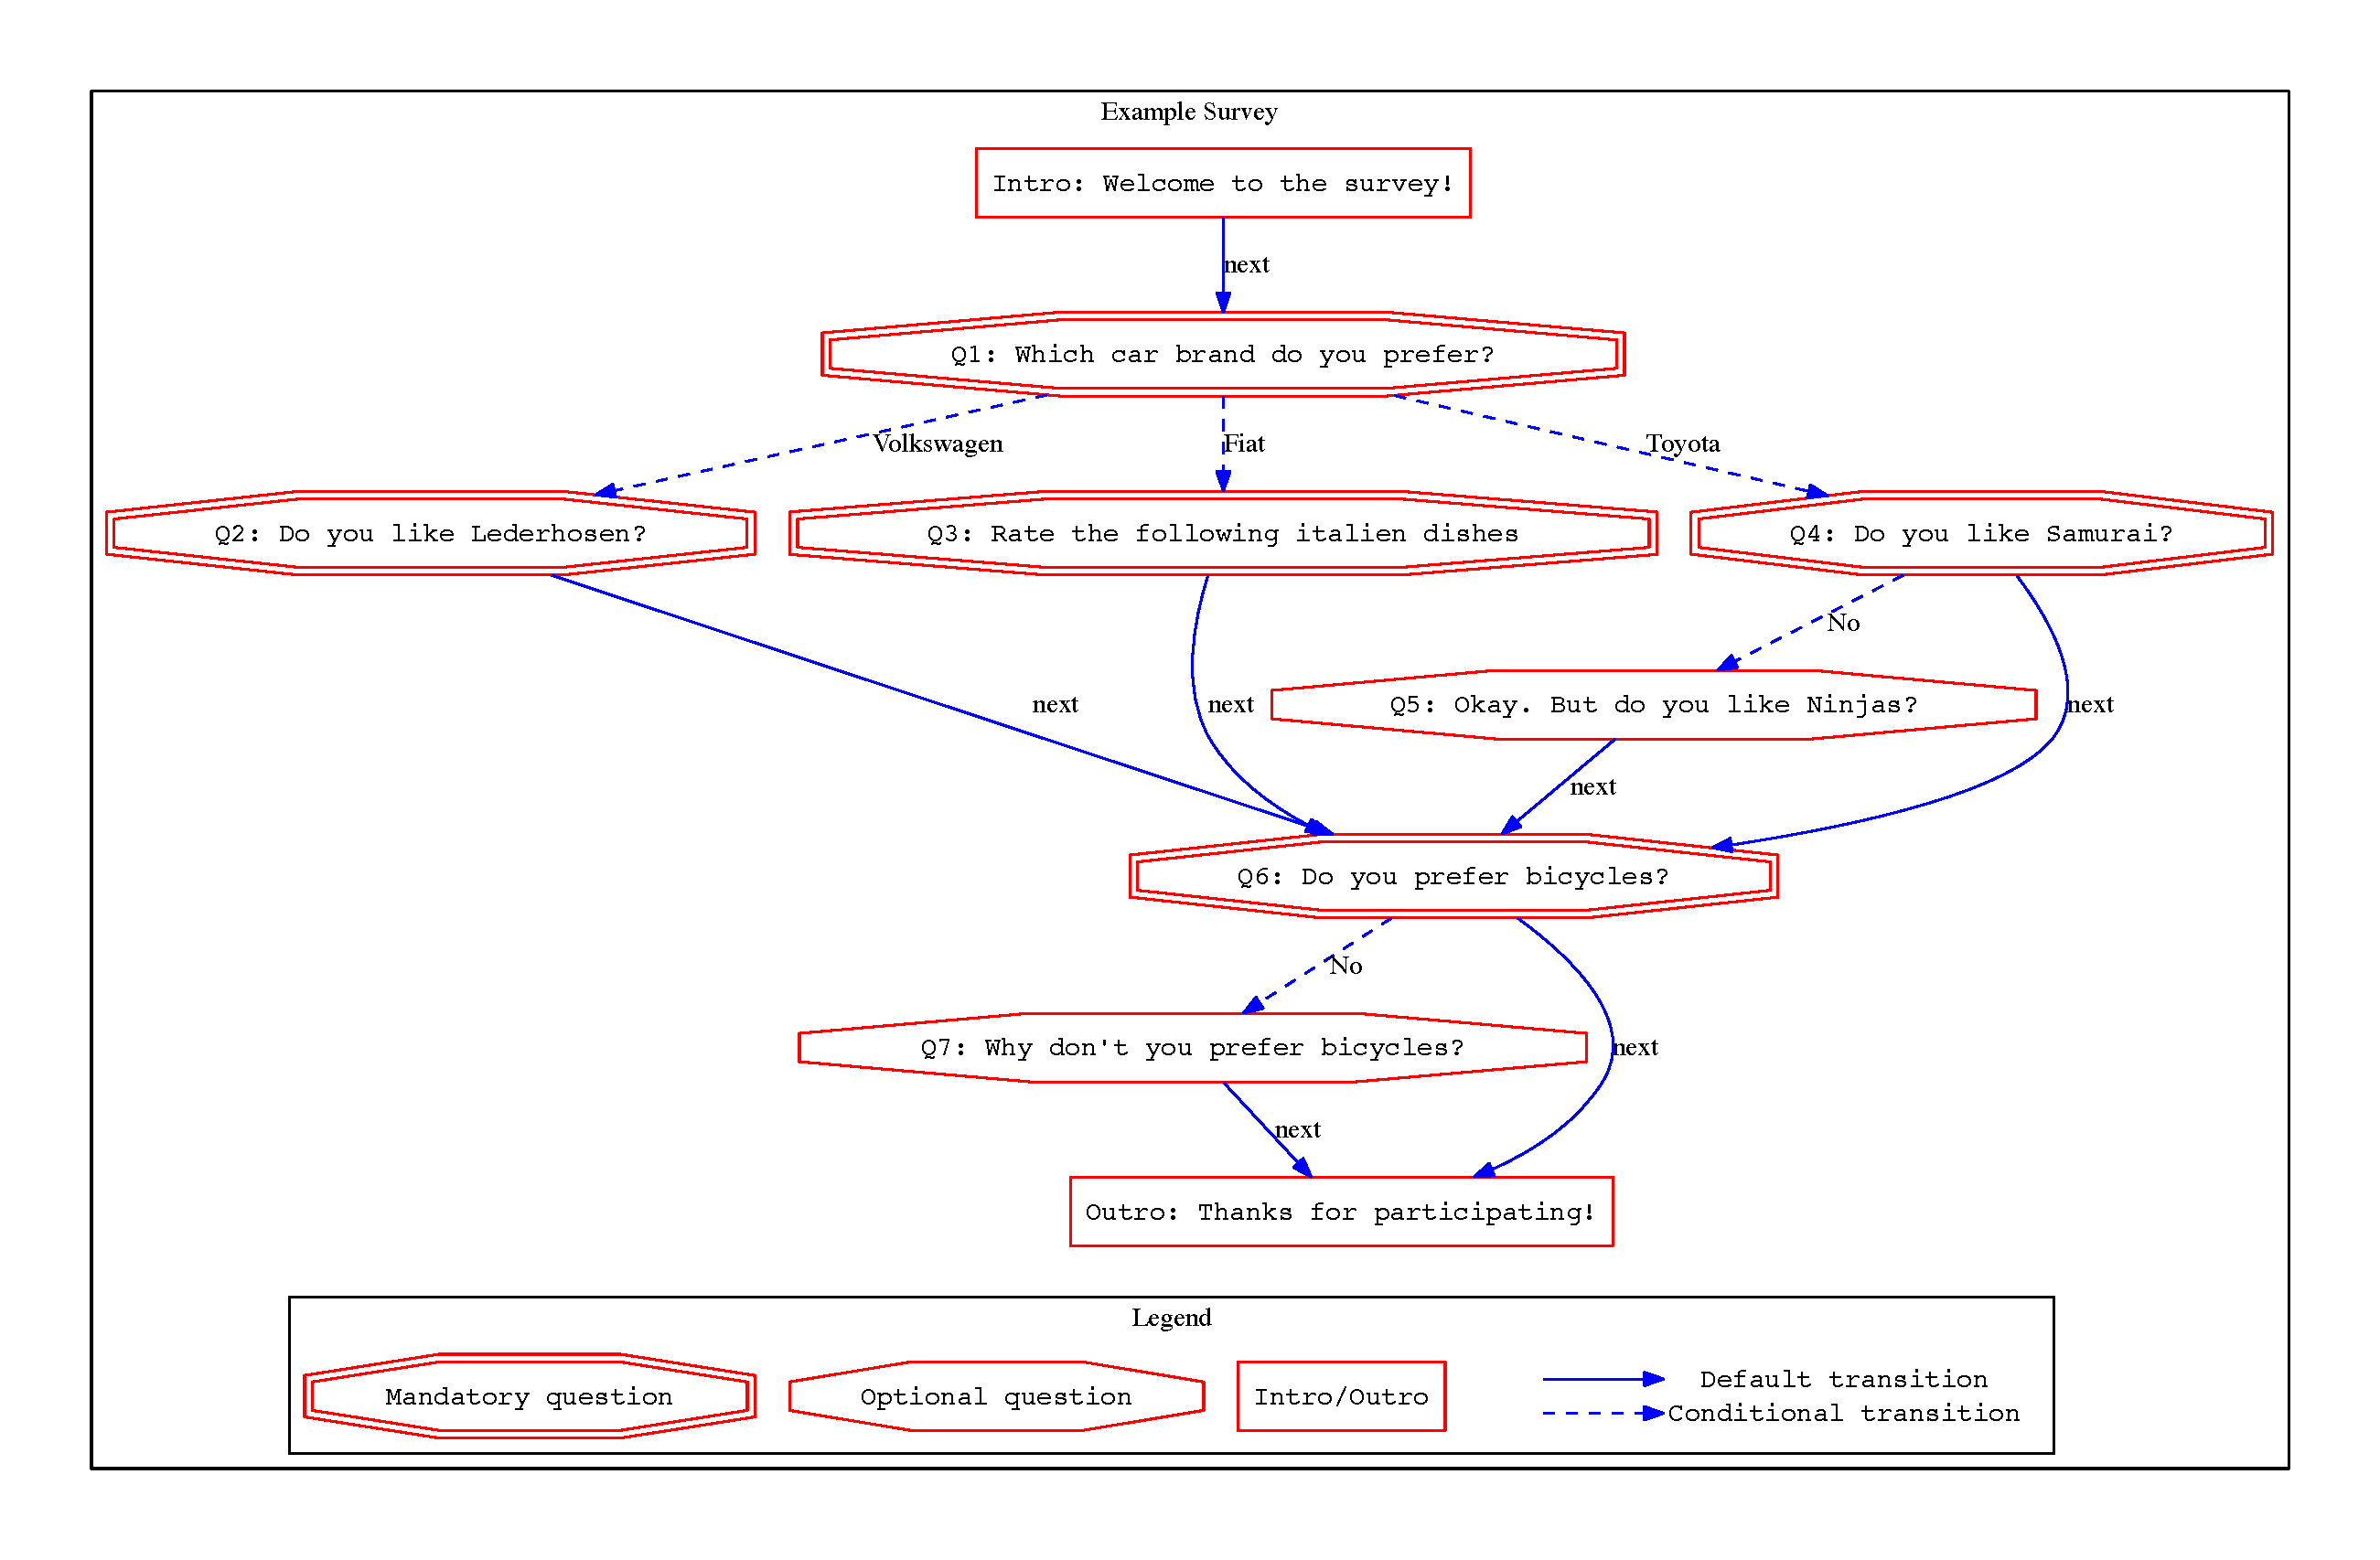
\includegraphics[scale=0.50,angle=270]{images/graph_example_survey}
	\caption{Generated DOT graph}
	\label{fig:survey_graph}
\end{figure}

\newpage
\begin{figure}[htb]
\begin{lstlisting}[language=survey]
Survey "SurveyApp"

Intro "Welcome to this awesome survey!"

Question Q1 exclusive "Do you want to build a snowman?" (
	Answer "Yes"
	Answer "No"
	Answer "Go away Anna!"
	Answer freetext "Other:"
)

Question Q2 "What is your quest?" (
	Answer "To burn bananas"
	Answer "To seek the Holy Grail" -> Q3, Q4
	Answer "I don't know" -> Q3
	Answer freetext "Other"
)

Question Q3 optional "What is the airspeed velocity of an unladen swallow?" (
	Answer "10 km/h"
	Answer "African or European?"
	Answer "2 teemos"
)

TableQuestion Q4 exclusive "How good are these things?" (
	Items ("Chocolate", "Chips", "Beer", freetext "Other")
	Answer "Bad"
	Answer "Average"
	Answer "Good"
	Answer "Excellent"
)

TableQuestion Q5 exclusive optional "How good are these things 2?" (
	Items ("Milk", "Apple", "Fish", freetext "Other")
	Answer "Bad"
	Answer "Average"
	Answer "Good"
	Answer "Excellent"
)

Question Q6 "Any other comments?" (
	Answer freetext ""
)

Outro "This is the end of the survey! Bye!"
\end{lstlisting}
\caption{A survey example for generating Android app}
\label{fig:survey_example_android}
\end{figure}

\begin{figure}[htb]
	\centering
	\subfigure[Intro]{
	
\includegraphics[scale=0.22]{images/android/android_0}}
	\quad
	\subfigure[Question 1]{
	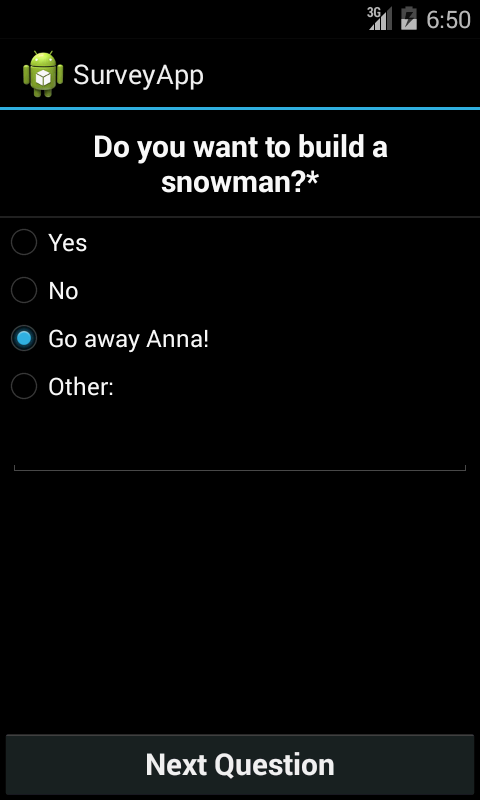
\includegraphics[scale=0.22]{images/android/android_1}}
	\subfigure[Question 2]{
	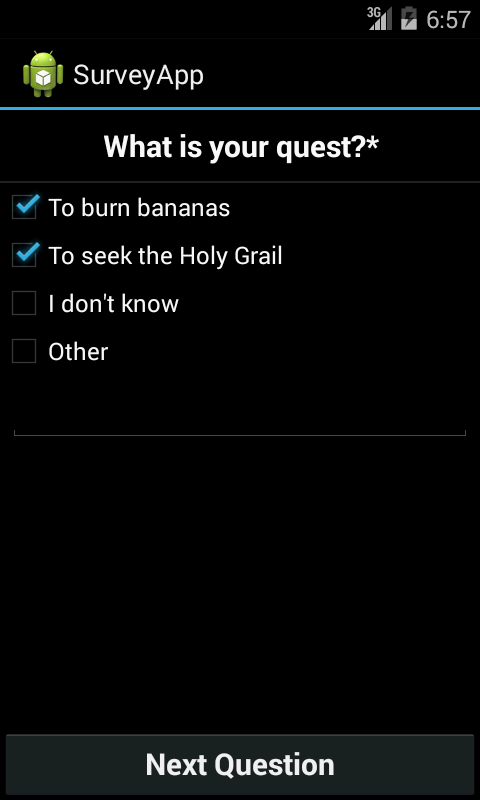
\includegraphics[scale=0.22]{images/android/android_2}}
	\quad
	\subfigure[Question 3]{
	
\includegraphics[scale=0.22]{images/android/android_3}}
	\subfigure[Question 4]{
	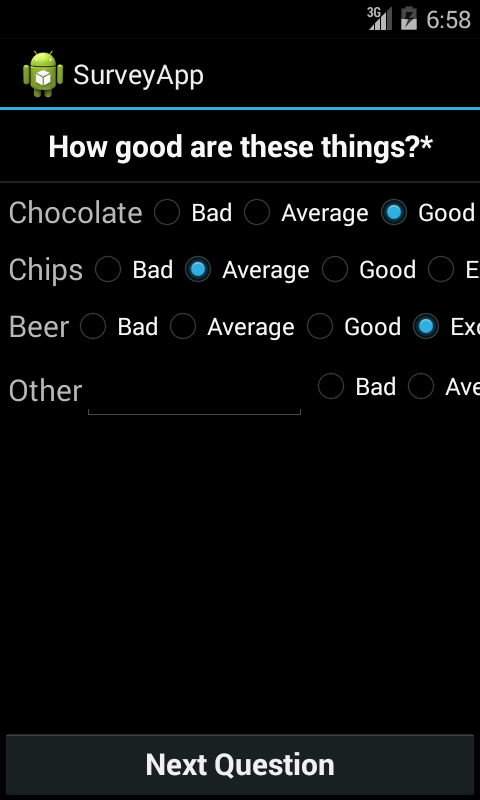
\includegraphics[scale=0.22]{images/android/android_4}}
	\quad
	\subfigure[Question 5]{
	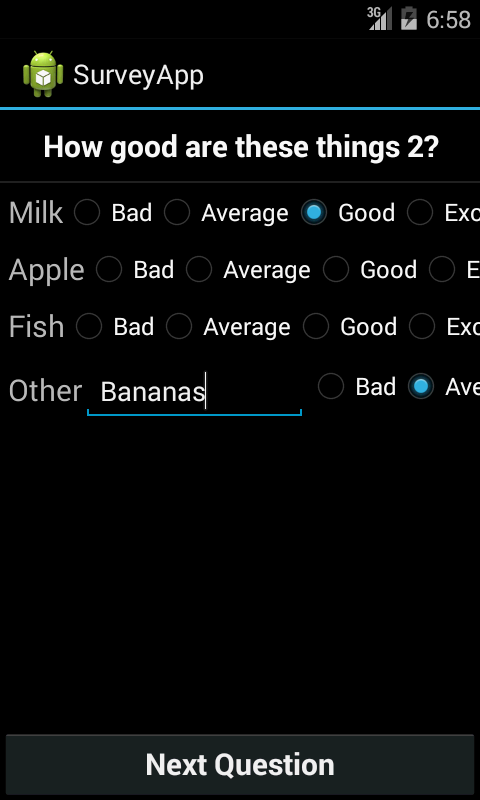
\includegraphics[scale=0.22]{images/android/android_5}}
	\subfigure[Question 6]{
	
\includegraphics[scale=0.22]{images/android/android_6}}
	\quad
	\subfigure[Outro]{
	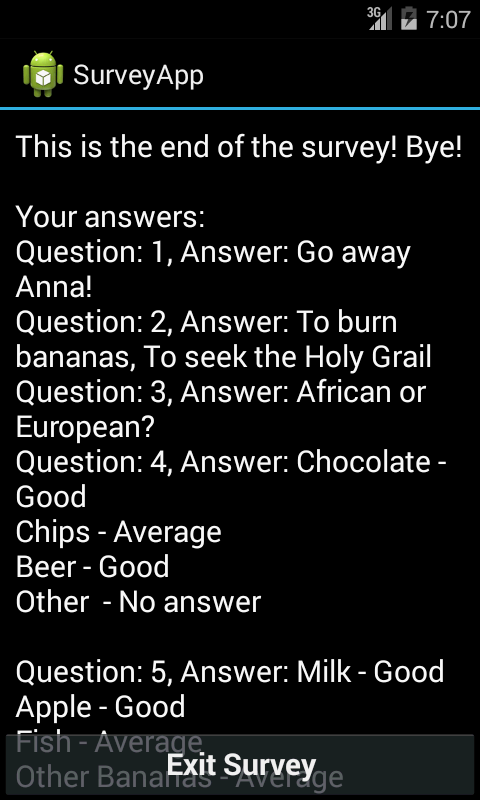
\includegraphics[scale=0.22]{images/android/android_7}}
	\caption{Generated Android app}
	\label{fig:android_app}
\end{figure}

\end{document}